\begin{center}
\section{Evaluation}
\label{sec:eval}
\end{center}

The project can be evaluated on its software engineering achievement(Section\ref{sec:system}) and the proposed SLACIH and DLACIH algorithm performance(Section\ref{method}); each has its challenges, with clear goals and strategies outlined. The evaluation in this section has been backed up with evidence of data in achieving the goals.

\subsection{Functional \& Non-Functional Requirements}

For the software engineering achievements, precise requirements were set in the functional and non-functional requirements(Section\ref{sec:requirements}). 
 The requirements in Table\ref{tab:functionalreq}\&\ref{tab:nonfunctionalreq} have been evaluated with what has been achieved in the Tables\ref{tab:functionalachieved}\&\ref{tab:nonfunctionalachieved}: 

\begin{table}[H]
    \centering
    \renewcommand{\arraystretch}{1.2} % Adjust row height for readability
    \begin{tabularx}{\textwidth}{|p{4cm}|X|}
\hline
\multicolumn{1}{|c|}{{\ul \textbf{Requirement}}} & \multicolumn{1}{c|}{{\ul \textbf{Achieved}}} \\ \hline
1.a) Graph Theory                              &  Two-dimensional graphs are represented in \href{https://github.com/AndrewF001/Dissertation/blob/main/TSP_Solution/TSP_Library/tsp_data/types/2d.h}{2d.h} and tested     \\ \hline
1.b) TSP Constraints                           &  \href{https://github.com/AndrewF001/Dissertation/blob/main/TSP_Solution/TSP_Library/tsp_data/tsp_data_template.h}{tsp\_data\_template.h} correctly enforces the constraints of the Travelling Salesman Problem     \\ \hline
1.c) Euclidean TSP                             &  The $getDistance()$ function correctly calculates the Euclidean distance  \\ \hline
 \makecell[l]{2.a) Facilities for \\ Algorithms}                  &  \href{https://github.com/AndrewF001/Dissertation/blob/main/TSP_Solution/TSP_Library/tsp_template.h}{tsp\_template.h} allows multiple algorithms to be used simply by changing a variable value   \\ \hline
 \makecell[l]{2.b) Benchmarking \\ Algorithm}                     &   \href{https://github.com/AndrewF001/Dissertation/blob/main/TSP_Solution/Utilities/timer.h}{timer.h} is a custom-built high-resolution clock timer specifically built for this project, and extended \href{https://github.com/AndrewF001/Dissertation/blob/main/TSP_Solution/TSP_Library/file_handling/tsp_structs.h}{tsp\_file} to include all the information needed\\ \hline
2.c) Algorithm Fairness                        &   The use of compile-time polymorphism treats every algorithm as individual sets of code, each being inlined and optimised by the compiler without knowledge of the other algorithm, and each algorithm worked with the same API calls and features\\ \hline
2.d) Testing Suite                             &  There are 5 test suites(Table\ref{tab:testsuites}), and developed on a \href{https://github.com/AndrewF001/Dissertation/blob/main/TSP_Solution/Empirical_Testing/Tests/test_class.h}{stable testing platform}                                          \\ \hline
 \makecell[l]{3.a) Display TSP \\ Solutions}                     &  There is a GUI application for displaying one or many TSP solutions \\ \hline
4.a) Collect Test Data                         &  TSP files with test data are created in JSON format \\ \hline
4.b) Analysis Test Data                        &  Excel tables and graphs and programmatically produced from the TSP files   \\ \hline
5.a) Unit Test                                 &  The unit tests covers TSP\_Library but not all aspects all aspects of the code base  \\ \hline
    \end{tabularx}
    \caption{Functional Requirements Achieved}
    \label{tab:functionalachieved}
\end{table}

\begin{table}[H]
    \centering
    \renewcommand{\arraystretch}{1.2} % Adjust row height for readability
    \begin{tabularx}{\textwidth}{|X|X|}
    \hline
{\ul \textbf{Requirement}}                                                                         & {\ul \textbf{Achieved}} \\ \hline
The user should be able to select the type of algorithm they want easily                   & The user can efficiently run pre-made algorithm setups, however, because compile-time polymorphism requires knowledge of which algorithm will be run beforehand, unless the user is a programmer, they are unlikely able to configure the bespoke algorithm            \\ \hline
The program should never fail or crash                                                     & The testing suites were run for multiple days without a crash or invalid TSP solution          \\ \hline
The program should be responsive and utilise all computing power                           & The program does not hang and uses all available cores when running multiple solutions         \\ \hline
The program should be adaptable and fill the needs of each executable                      & There is no repeated code to cover the same functionality       \\ \hline
The GUI should be easy to read for all users e.g. inclusive of those with colour blindness &      The colour palette does not clash with common colour blindness, but the graphics are small and lack graphical fidelity features like anti-aliasing             \\ \hline
    \end{tabularx}
    \caption{Non-Functional Requirements Achieved}
    \label{tab:nonfunctionalachieved}
\end{table}
\pagebreak
\subsection{Empirical Testing Results}

Following this report's research, methodology, design and testing; empirical testing is the lead evaluation for comparing the Static \& Dynamic Look-Ahead Cheapest Insertion Heuristic against other known heuristics. Every algorithm(Table\ref{tab:algacry}) used Quad-Tree Partitioning, Full Caching, and tour optimiser with 2-opt swap, because from testing this was shown to be the best set-up for solution result and run time.

\begin{table}[H]
    \centering
    \renewcommand{\arraystretch}{1.2} % Adjust row height for readability
    \begin{tabularx}{\textwidth}{|p{2.5cm}|X|}
    \hline
      \textbf{Acronym}   & \textbf{Algorithm} \\
      \hline
        DLACHCIH & Dynamic Look-Ahead Convex Hull Cheapest Insertion Heuristic\\
        DLACIH & Dynamic Look-Ahead Cheapest Insertion Heuristic \\
        SLACHCIH(X) & Static Look-Ahead Convex Hull Cheapest Insertion Heuristic, Depth = X\\
        SLACIH(X) & Static Look-Ahead Cheapest Insertion Heuristic, Depth = X \\
        NNS & Nearest Neighbour Search Heuristic \\
        CHCIH & Convex Hull Cheapest Insertion Heuristic \\
        CIH & Cheapest Insertion Heuristic \\
        \hline
    \end{tabularx}
    \caption{Algorithm Acronym Key}
    \label{tab:algacry}
\end{table}

Each test instance problem was randomly generated. and ran on each algorithm for six problem sizes, which were chosen to represent small, medium, and large problems. Multiple depths of the static look-ahead were evaluated to prove and develop the dynamic look-ahead optimal depth curvature. \label{test:dynamic}This report theorised lots of dynamic algorithms(Section\ref{Dynamic}), but for this testing, only static dynamic depth optimisation(Section\ref{SDynamic}) was considered. As DLACIH calls upon SLACIH code and therefore would generate the same solution, running the code twice was avoided to speed up testing. The distance values for DLACIH and DLACHCIH are based on the static depth it would have chosen to run SLACIH, and the times can be assumed to be identical, but left blank for clarity.

Each value in the Table\ref{tab:DistanceResult}\&\ref{tab:TimeResult} is the mean average of 1,000 problems being solved. This results in 114,000 TSP problems being solved and 240,540,000 Nodes being routed. This required multiple weeks of constant computational running and tens of thousands of CPU hours.

\begin{landscape}
% \pagebreak
% \begin{table}
%   \centering
%   \setlength\tabcolsep{0pt}
%   \begin{tabular*}{\linewidth}{@{\extracolsep{\fill}}
%                         |p{3cm}|
%                    *{2}{S[table-format= 1.5]}|
%                    *{2}{S[table-format= 1.5]}|
%                    *{2}{S[table-format= 1.5]}|
%                    *{2}{S[table-format= 1.5]}|
%                    *{2}{S[table-format= 1.5]}|
%                    *{2}{S[table-format= 1.5]}|
%                             } 
%     \toprule 
    
%      & \multicolumn{12}{c}{\textbf{Problem Size}}\\
%      &   \multicolumn{2}{c}{10 Nodes}   &   \multicolumn{2}{c}{100 Nodes}  &\multicolumn{2}{c}{200 Nodes}  &\multicolumn{2}{c}{300 Nodes}  &\multicolumn{2}{c}{500 Nodes}  &\multicolumn{2}{c}{1000 Nodes}   \\
%     \midrule
%     {\textbf{Algorithm}}&   {\thead[b]{Distance}} &   {\thead[b]{Time}}
%     &   {\thead[b]{Distance}} &   {\thead[b]{Time}}
%     &   {\thead[b]{Distance}} &   {\thead[b]{Time}}
%     &   {\thead[b]{Distance}} &   {\thead[b]{Time}}
%     &   {\thead[b]{Distance}} &   {\thead[b]{Time}}
%     &   {\thead[b]{Distance}} &   {\thead[b]{Time}}\\
%     \midrule
% {DLACHCIH}       & {0.123}    & {1.234} & {0.12}     & {0.123}    & {0.123} & {0.123} & {1.234} & {1.234} & {1.234} & {1.234} & {1.234} & {1.234}        \\ 
% \myrowcolour%
% {DLACIH}         & {0.123}    & {1.234} & {0.12}     & {0.123}    & {0.123} & {0.123} & {1.234} & {1.234} & {1.234} & {1.234} & {1.234} & {1.234}        \\ 
% {SLACHCIH(0)} & {2864.35} & {28.83} & {8191.25} & {5051.86} & {11490.84} & {36190.85} & {14062.30} & {111427.81} & {18156.44} & {488391.94} & {25651.97} & {3620307.70} \\
% \myrowcolour%
% {SLACHCIH(1)} & {2864.57} & {25.37} & {8151.50} & {7261.49} & {11433.55} & {48326.42} & {13988.46} & {155657.94} & {18049.47} & {689855.24} & {25467.84} & {6353401.04} \\
% {SLACHCIH(2)} & {2864.46} & {24.09} & {8140.39} & {8234.30} & {11398.91} & {56582.62} & {13939.97} & {182868.75} & {17964.59} & {803808.43} & {25327.55} & {7537333.35} \\
% \myrowcolour%
% {SLACHCIH(3)} & {2864.55} & {24.06} & {8138.31} & {10040.87} & {11396.14} & {69633.18} & {13908.57} & {218068.36} & {17920.81} & {969888.68} & {25256.85} & {9223702.34} \\
% {SLACHCIH(4)} & {2864.47} & {24.41} & {8143.77} & {12184.33} & {11385.62} & {87280.23} & {13900.00} & {272952.20} & {17891.36} & {1220761.27} & {25210.99} & {11632562.85} \\
% \myrowcolour%
% {SLACHCIH(5)} & {2864.45} & {24.44} & {8150.61} & {14956.88} & {11394.39} & {108331.81} & {13902.06} & {343997.62} & {17895.56} & {1542499.09} & {25180.95} & {14895643.66} \\
% {SLACHCIH(6)} & {2864.45} & {24.71} & {8162.80} & {17467.33} & {11398.80} & {134173.32} & {13906.92} & {432163.16} & {17917.52} & {1968387.66} & {25177.56} & {19003165.87} \\
% \myrowcolour%
% {SLACHCIH(7)} & {2864.45} & {24.18} & {8173.54} & {20843.73} & {11418.06} & {164704.99} & {13933.31} & {533267.40} & {17916.94} & {2469852.32} & {25184.09} & {23702107.36} \\
% {SLACIH(0)} & {2898.15} & {39.98} & {8620.55} & {7902.99} & {11990.80} & {52819.91} & {14581.91} & {155816.52} & {18717.76} & {646409.43} & {26242.28} & {4608439.04} \\
% \myrowcolour%
% {SLACIH(1)} & {2886.81} & {43.13} & {8540.03} & {9994.76} & {11885.12} & {65427.01} & {14441.23} & {205581.55} & {18530.75} & {879891.38} & {25998.57} & {7931265.55} \\
% {SLACIH(2)} & {2885.52} & {42.97} & {8480.63} & {10616.85} & {11783.13} & {68674.72} & {14343.36} & {216557.75} & {18401.00} & {934354.74} & {25802.91} & {8607775.94} \\
% \myrowcolour%
% {SLACIH(3)} & {2878.55} & {45.30} & {8420.75} & {11922.03} & {11721.57} & {76106.33} & {14256.36} & {238098.60} & {18302.12} & {1034565.22} & {25658.64} & {9749928.92} \\
% {SLACIH(4)} & {2878.31} & {49.89} & {8373.10} & {13914.21} & {11685.38} & {88204.19} & {14199.79} & {271463.36} & {18232.74} & {1200665.81} & {25545.87} & {11465799.93} \\
% \myrowcolour%
% {SLACIH(5)} & {2877.51} & {52.51} & {8363.03} & {15820.59} & {11651.66} & {104870.35} & {14152.21} & {333552.41} & {18176.34} & {1444295.09} & {25488.85} & {13928589.28} \\
% {SLACIH(6)} & {2874.40} & {59.00} & {8343.51} & {19406.64} & {11628.51} & {127248.89} & {14132.63} & {394223.06} & {18149.98} & {1762965.96} & {25436.01} & {17155433.92} \\
% \myrowcolour%
% {SLACIH(7)} & {2873.75} & {58.87} & {8336.78} & {22896.07} & {11605.18} & {154385.62} & {14121.65} & {479555.42} & {18118.21} & {2168896.75} & {25419.93} & {21146002.81} \\
% {NNS} & {2888.89} & {51.85} & {8494.45} & {8163.56} & {11828.17} & {53758.76} & {14379.98} & {160573.75} & {18451.89} & {664739.17} & {25847.28} & {4624162.49} \\
% \myrowcolour%
% {CHCIH} & {2864.35} & {74.79} & {8190.42} & {16037.53} & {11492.43} & {61741.36} & {14063.86} & {173547.76} & {18147.45} & {694579.49} & {25581.89} & {4909795.79} \\
% {CIH} & {2898.15} & {39.75} & {8619.66} & {7892.48} & {11991.10} & {53696.50} & {14571.81} & {158542.26} & {18678.65} & {674338.86} & {26132.84} & {4904754.48} \\
%  \bottomrule
%   \end{tabular*}
%   \begin{tablenotes}[flushleft]\small
%   \source: Average of 1000 random problems
%   \note:   Red values are best in class
%   \end{tablenotes}
%   \caption{Empirical Testing Results }\label{tab:results2}
% \end{table}

{\captionsetup{font=Large, labelsep=space}
% \begin{table}
%   \centering
%   \caption{Empirical Testing Distance Results }\label{tab:DistanceResult}
%   \setlength\tabcolsep{0pt}
%   \begin{tabular*}{\linewidth}{@{\extracolsep{\fill}}
%                 |p{3cm}|p{3cm}|p{3cm}|p{3cm}|p{3cm}|p{3cm}|p{3cm}|
%                    % *{6}{S[table-format= 1.5]}|
%                             } 
%     \toprule 
%      & \multicolumn{5}{c}{\textbf{Problem Size}} \\
%      \cmidrule[0.4pt](r{0.125em}){2-7}%
%      {\textbf{Algorithm}} &  {10 Nodes}   &  {100 Nodes}  & {200 Nodes}  & {300 Nodes}  & {500 Nodes}  & {1000 Nodes}   \\
%     \midrule

% \ DLACHCIH & \highest{2864.35} & \highest{8138.31} & \highest{11385.62} & 13902.06 & 17895.56 & 25180.95 \\
% \myrowcolour
% \ DLACIH & 2898.15 & 8420.75 & 11685.38 & 14256.36 & 18176.34 & 25436.01 \\
% \ SLACHCIH(0) & \highest{2864.35} & 8191.25 & 11490.84 & 14062.30 & 18156.44 & 25651.97 \\
% \myrowcolour
% \ SLACHCIH(1) & 2864.57 & 8151.50 & 11433.55 & 13988.46 & 18049.47 & 25467.84 \\
% \ SLACHCIH(2) & 2864.46 & 8140.39 & 11398.91 & 13939.97 & 17964.59 & 25327.55 \\
% \myrowcolour
% \ SLACHCIH(3) & 2864.55 & \highest{8138.31} & 11396.14 & 13908.57 & 17920.81 & 25256.85 \\
% \ SLACHCIH(4) & 2864.47 & 8143.77 & \highest{11385.62} & \highest{13900.00} & \highest{17891.36} & 25210.99 \\
% \myrowcolour
% \ SLACHCIH(5) & 2864.45 & 8150.61 & 11394.39 & 13902.06 & 17895.56 & 25180.95 \\
% \ SLACHCIH(6) & 2864.45 & 8162.80 & 11398.80 & 13906.92 & 17917.52 & \highest{25177.56} \\
% \myrowcolour
% \ SLACHCIH(7) & 2864.45 & 8173.54 & 11418.06 & 13933.31 & 17916.94 & 25184.09 \\
% \ SLACIH(0)  & 2898.15 & 8620.55 & 11990.80 & 14581.91 & 18717.76 & 26242.28 \\
% \myrowcolour
% \ SLACIH(1)  & 2886.81 & 8540.03 & 11885.12 & 14441.23 & 18530.75 & 25998.57 \\
% \ SLACIH(2)  & 2885.52 & 8480.63 & 11783.13 & 14343.36 & 18401.00 & 25802.91 \\
% \myrowcolour
% \ SLACIH(3)  & 2878.55 & 8420.75 & 11721.57 & 14256.36 & 18302.12 & 25658.64 \\
% \ SLACIH(4)  & 2878.31 & 8373.10 & 11685.38 & 14199.79 & 18232.74 & 25545.87 \\
% \myrowcolour
% \ SLACIH(5)  & 2877.51 & 8363.03 & 11651.66 & 14152.21 & 18176.34 & 25488.85 \\
%  \scalebox{0.85}{ SLACIH(6)  & 2874.40 & 8343.51 & 11628.51 & 14132.63 & 18149.98 & 25436.01 \\
% \myrowcolour
% \ SLACIH(7)  & 2873.75 & 8336.78 & 11605.18 & 14121.65 & 18118.21 & 25419.93 \\
% \ NNS         & 2888.89 & 8494.45 & 11828.17 & 14379.98 & 18451.89 & 25847.28 \\
% \myrowcolour
% \ CHCIH       & 2864.35 & 8190.42 & 11492.43 & 14063.86 & 18147.45 & 25581.89 \\
% \ CIH         & 2898.15 & 8619.66 & 11991.10 & 14571.81 & 18678.65 & 26132.84 \\
%  \bottomrule
%   \end{tabular*}
%   \begin{tablenotes}[flushleft]\small
%   \source: Average of 1000 random problems
%   \note:   Red values are best in class
%   \end{tablenotes}
% \end{table}

\begin{table}[]
  \centering
  \caption{\\ Empirical Testing Distance Results }\label{tab:DistanceResult}
\resizebox{0.9\linewidth}{!}{%
\begin{tabular}{|c|cccccc|}
\hline
                                     & \multicolumn{6}{c|}{\textbf{Problem Size}}                                                                                                                                                              \\ \cline{2-7} 
\multirow{-2}{*}{\textbf{Algorithm}} & \multicolumn{1}{l|}{10 Nodes}  & \multicolumn{1}{l|}{100 Nodes} & \multicolumn{1}{l|}{200 Nodes}  & \multicolumn{1}{l|}{300 Nodes}  & \multicolumn{1}{l|}{500 Nodes}  & \multicolumn{1}{l|}{1000 Nodes} \\ \hline
\textbf{DLACHCIH}                    & {\color[HTML]{FE0000} 2864.35} & {\color[HTML]{FE0000} 8138.31} & {\color[HTML]{FE0000} 11385.62} & 13902.06                        & 17895.56                        & 25180.95                        \\
\rowcolor[HTML]{EFEFEF} 
\textbf{DLACIH}                      & 2898.15                        & 8420.75                        & 11685.38                        & 14256.36                        & 18176.34                        & 25436.01                        \\
\textbf{SLACHCIH(0)}                 & {\color[HTML]{FE0000} 2864.35} & 8191.25                        & 11490.84                        & 14062.30                        & 18156.44                        & 25651.97                        \\
\rowcolor[HTML]{EFEFEF} 
\textbf{SLACHCIH(1)}                 & 2864.57                        & 8151.50                        & 11433.55                        & 13988.46                        & 18049.47                        & 25467.84                        \\
\textbf{SLACHCIH(2)}                 & 2864.46                        & 8140.39                        & 11398.91                        & 13939.97                        & 17964.59                        & 25327.55                        \\
\rowcolor[HTML]{EFEFEF} 
\textbf{SLACHCIH(3)}                 & 2864.55                        & {\color[HTML]{FE0000} 8138.31} & 11396.14                        & 13908.57                        & 17920.81                        & 25256.85                        \\
\textbf{SLACHCIH(4)}                 & 2864.47                        & 8143.77                        & {\color[HTML]{FE0000} 11385.62} & {\color[HTML]{FE0000} 13900.00} & {\color[HTML]{FE0000} 17891.36} & 25210.99                        \\
\rowcolor[HTML]{EFEFEF} 
\textbf{SLACHCIH(5)}                 & 2864.45                        & 8150.61                        & 11394.39                        & 13902.06                        & 17895.56                        & 25180.95                        \\
\textbf{SLACHCIH(6)}                 & 2864.45                        & 8162.80                        & 11398.80                        & 13906.92                        & 17917.52                        & {\color[HTML]{FE0000} 25177.56} \\
\rowcolor[HTML]{EFEFEF} 
\textbf{SLACHCIH(7)}                 & 2864.45                        & 8173.54                        & 11418.06                        & 13933.31                        & 17916.94                        & 25184.09                        \\
\textbf{SLACIH(0)}                   & 2898.15                        & 8620.55                        & 11990.80                        & 14581.91                        & 18717.76                        & 26242.28                        \\
\rowcolor[HTML]{EFEFEF} 
\textbf{SLACIH(1)}                   & 2886.81                        & 8540.03                        & 11885.12                        & 14441.23                        & 18530.75                        & 25998.57                        \\
\textbf{SLACIH(2)}                   & 2885.52                        & 8480.63                        & 11783.13                        & 14343.36                        & 18401.00                        & 25802.91                        \\
\rowcolor[HTML]{EFEFEF} 
\textbf{SLACIH(3)}                   & 2878.55                        & 8420.75                        & 11721.57                        & 14256.36                        & 18302.12                        & 25658.64                        \\
\textbf{SLACIH(4)}                   & 2878.31                        & 8373.10                        & 11685.38                        & 14199.79                        & 18232.74                        & 25545.87                        \\
\rowcolor[HTML]{EFEFEF} 
\textbf{SLACIH(5)}                   & 2877.51                        & 8363.03                        & 11651.66                        & 14152.21                        & 18176.34                        & 25488.85                        \\
\textbf{SLACIH(6)}                   & 2874.40                        & 8343.51                        & 11628.51                        & 14132.63                        & 18149.98                        & 25436.01                        \\
\rowcolor[HTML]{EFEFEF} 
\textbf{SLACIH(7)}                   & 2873.75                        & 8336.78                        & 11605.18                        & 14121.65                        & 18118.21                        & 25419.93                        \\
\textbf{NNS}                         & 2888.89                        & 8494.45                        & 11828.17                        & 14379.98                        & 18451.89                        & 25847.28                        \\
\rowcolor[HTML]{EFEFEF} 
\textbf{CHCIH}                       & 2864.35                        & 8190.42                        & 11492.43                        & 14063.86                        & 18147.45                        & 25581.89                        \\
\textbf{CIH}                         & 2898.15                        & 8619.66                        & 11991.10                        & 14571.81                        & 18678.65                        & 26132.84                        \\ \hline
\end{tabular}%
}
  \begin{tablenotes}[flushleft]\small
  \source: Average of 1000 random problems
  \note:   Red values are best in class
  \end{tablenotes}
\end{table}

\pagebreak
% \begin{table}
%   \centering
%   \caption{Empirical Testing Time(Microseconds) Results}\label{tab:TimeResult}
%   \setlength\tabcolsep{0pt}
%     \begin{tabular*}{\linewidth}{@{\extracolsep{\fill}}
%                 |p{3cm}|p{3cm}|p{3cm}|p{3cm}|p{3cm}|p{3cm}|p{3cm}|
%                    % *{6}{S[table-format= 1.5]}|
%                             } 
%     \toprule 
%      & \multicolumn{5}{c}{\textbf{Problem Size}} \\
%      \cmidrule[0.4pt](r{0.125em}){2-7}%
%      {\textbf{\ Algorithm}} &  {10 Nodes}   &  {100 Nodes}  & {200 Nodes}  & {300 Nodes}  & {500 Nodes}  & {1000 Nodes}   \\
%     \midrule

% \ DLACHCIH & N/A & N/A & N/A & N/A & N/A & N/A \\
% \myrowcolour
% \ DLACIH & N/A & N/A & N/A & N/A & N/A & N/A \\
% \ SLACHCIH(0) & 28.83 & 5051.86 & 36190.85 & 111427.81 & 488391.94 & 3620307.70 \\
% \myrowcolour
% \ SLACHCIH(1) & 25.37 & 7261.49 & 48326.42 & 155657.94 & 689855.24 & 6353401.04 \\
% \ SLACHCIH(2) & 24.09 & 8234.30 & 56582.62 & 182868.75 & 803808.43 & 7537333.35 \\
% \myrowcolour
% \ SLACHCIH(3) & 24.06 & 10040.87 & 69633.18 & 218068.36 & 969888.68 & 9223702.34 \\
% \ SLACHCIH(4) & 24.41 & 12184.33 & 87280.23 & 272952.20 & 1220761.27 & 11632562.85 \\
% \myrowcolour
% \ SLACHCIH(5) & 24.44 & 14956.88 & 108331.81 & 343997.62 & 1542499.09 & 14895643.66 \\
% \ SLACHCIH(6) & 24.71 & 17467.33 & 134173.32 & 432163.16 & 1968387.66 & 19003165.87 \\
% \myrowcolour
% \ SLACHCIH(7) & 24.18 & 20843.73 & 164704.99 & 533267.40 & 2469852.32 & 23702107.36 \\
% \ SLACIH(0)  & 39.98 & 7902.99 & 52819.91 & 155816.52 & 646409.43 & 4608439.04 \\
% \myrowcolour
% \ SLACIH(1)  & 43.13 & 9994.76 & 65427.01 & 205581.55 & 879891.38 & 7931265.55 \\
% \ SLACIH(2)  & 42.97 & 10616.85 & 68674.72 & 216557.75 & 934354.74 & 8607775.94 \\
% \myrowcolour
% \ SLACIH(3)  & 45.30 & 11922.03 & 76106.33 & 238098.60 & 1034565.22 & 9749928.92 \\
% \ SLACIH(4)  & 49.89 & 13914.21 & 88204.19 & 271463.36 & 1200665.81 & 11465799.93 \\
% \myrowcolour
% \ SLACIH(5)  & 52.51 & 15820.59 & 104870.35 & 333552.41 & 1444295.09 & 13928589.28 \\
% \ SLACIH(6)  & 59.00 & 19406.64 & 127248.89 & 394223.06 & 1762965.96 & 17155433.92 \\
% \myrowcolour
% \ SLACIH(7)  & 58.87 & 22896.07 & 154385.62 & 479555.42 & 2168896.75 & 21146002.81 \\
% \ NNS         & 51.85 & 8163.56 & 53758.76 & 160573.75 & 664739.17 & 4624162.49 \\
% \myrowcolour
% \ CHCIH       & 74.79 & 16037.53 & 61741.36 & 173547.76 & 694579.49 & 4909795.79 \\
% \ CIH         & 39.75 & 7892.48 & 53696.50 & 158542.26 & 674338.86 & 4904754.48 \\
%  \bottomrule
%   \end{tabular*}
%   \begin{tablenotes}[flushleft]\small
%   \source: Average of 1000 random problems
%   \end{tablenotes}
% \end{table}

% \pagebreak

\begin{table}[]
  \centering
  \caption{\\ Empirical Testing Time(Microseconds) Results}\label{tab:TimeResult}
\resizebox{0.9\linewidth}{!}{%
\begin{tabular}{|c|cccccc|}
\hline
                                     & \multicolumn{6}{c|}{\textbf{Problem Size}}                                                                                                                                                          \\ \cline{2-7} 
\multirow{-2}{*}{\textbf{Algorithm}} & \multicolumn{1}{l|}{10 Nodes} & \multicolumn{1}{l|}{100 Nodes} & \multicolumn{1}{l|}{200 Nodes} & \multicolumn{1}{l|}{300 Nodes} & \multicolumn{1}{l|}{500 Nodes} & \multicolumn{1}{l|}{1000 Nodes} \\ \hline
\textbf{DLACHCIH}                    & N/A                           & N/A                            & N/A                            & N/A                            & N/A                            & N/A                             \\
\rowcolor[HTML]{EFEFEF} 
\textbf{DLACIH}                      & N/A                           & N/A                            & N/A                            & N/A                            & N/A                            & N/A                             \\
\textbf{SLACHCIH(0)}                 & 28.83                         & 5051.86                        & 36190.85                       & 111427.81                      & 488391.94                      & 3620307.70                      \\
\rowcolor[HTML]{EFEFEF} 
\textbf{SLACHCIH(1)}                 & 25.37                         & 7261.49                        & 48326.42                       & 155657.94                      & 689855.24                      & 6353401.04                      \\
\textbf{SLACHCIH(2)}                 & 24.09                         & 8234.30                        & 56582.62                       & 182868.75                      & 803808.43                      & 7537333.35                      \\
\rowcolor[HTML]{EFEFEF} 
\textbf{SLACHCIH(3)}                 & 24.06                         & 10040.87                       & 69633.18                       & 218068.36                      & 969888.68                      & 9223702.34                      \\
\textbf{SLACHCIH(4)}                 & 24.41                         & 12184.33                       & 87280.23                       & 272952.20                      & 1220761.27                     & 11632562.85                     \\
\rowcolor[HTML]{EFEFEF} 
\textbf{SLACHCIH(5)}                 & 24.44                         & 14956.88                       & 108331.81                      & 343997.62                      & 1542499.09                     & 14895643.66                     \\
\textbf{SLACHCIH(6)}                 & 24.71                         & 17467.33                       & 134173.32                      & 432163.16                      & 1968387.66                     & 19003165.87                     \\
\rowcolor[HTML]{EFEFEF} 
\textbf{SLACHCIH(7)}                 & 24.18                         & 20843.73                       & 164704.99                      & 533267.40                      & 2469852.32                     & 23702107.36                     \\
\textbf{SLACIH(0)}                   & 39.98                         & 7902.99                        & 52819.91                       & 155816.52                      & 646409.43                      & 4608439.04                      \\
\rowcolor[HTML]{EFEFEF} 
\textbf{SLACIH(1)}                   & 43.13                         & 9994.76                        & 65427.01                       & 205581.55                      & 879891.38                      & 7931265.55                      \\
\textbf{SLACIH(2)}                   & 42.97                         & 10616.85                       & 68674.72                       & 216557.75                      & 934354.74                      & 8607775.94                      \\
\rowcolor[HTML]{EFEFEF} 
\textbf{SLACIH(3)}                   & 45.30                         & 11922.03                       & 76106.33                       & 238098.60                      & 1034565.22                     & 9749928.92                      \\
\textbf{SLACIH(4)}                   & 49.89                         & 13914.21                       & 88204.19                       & 271463.36                      & 1200665.81                     & 11465799.93                     \\
\rowcolor[HTML]{EFEFEF} 
\textbf{SLACIH(5)}                   & 52.51                         & 15820.59                       & 104870.35                      & 333552.41                      & 1444295.09                     & 13928589.28                     \\
\textbf{SLACIH(6)}                   & 59.00                         & 19406.64                       & 127248.89                      & 394223.06                      & 1762965.96                     & 17155433.92                     \\
\rowcolor[HTML]{EFEFEF} 
\textbf{SLACIH(7)}                   & 58.87                         & 22896.07                       & 154385.62                      & 479555.42                      & 2168896.75                     & 21146002.81                     \\
\textbf{NNS}                         & 51.85                         & 8163.56                        & 53758.76                       & 160573.75                      & 664739.17                      & 4624162.49                      \\
\rowcolor[HTML]{EFEFEF} 
\textbf{CHCIH}                       & 74.79                         & 16037.53                       & 61741.36                       & 173547.76                      & 694579.49                      & 4909795.79                      \\
\textbf{CIH}                         & 39.75                         & 7892.48                        & 53696.50                       & 158542.26                      & 674338.86                      & 4904754.48                      \\ \hline
\end{tabular}%
}
  \begin{tablenotes}[flushleft]\small
  \source: Average of 1000 random problems
  \end{tablenotes}
\end{table}
}
\pagebreak
\end{landscape}

For every problem size(Table\ref{tab:DistanceResult}), SLACHCIH provided the best solution from the algorithms tested, although the same depth was not used. As theorised, as the problem size increases, a higher look-ahead depth is optimal. This is where DLACHCIH's optimal depth function proved to be highly fit for purpose. However, the gradient descent variable optimisation failed to find the optimal curve that could otherwise be found through statistical analysis. The data also correctly demonstrated the theory that a higher depth is not always better. This is due to the pitfalls the look-ahead design introduces when it searches for nodes far away from a cluster(Section\ref{pitfall}).

From the conventional heuristic, CHCIH is the leading algorithm, but none could be better than DLACHCIH for any problem size. Using Equation\ref{eqt:resultcompar} to compare the solution results vs DLACHCIH in a Table\ref{tab:performance}: 
\begin{equation}
    \frac{\text{Conventional}_{Result}}{\text{DLACHCIH}_{Result}}-1
    \label{eqt:resultcompar}
\end{equation}


\begin{table}[H]
\caption{DLACHCIH vs Conventional Algorithm }\label{tab:performance}
\begin{tabular}{|l|llllll|l|}
\hline
\multirow{2}{*}{\textbf{\begin{tabular}[c]{@{}l@{}}Conventional\\ Algorithm\end{tabular}}} & \multicolumn{6}{c|}{\textbf{Problem Size}}                                                                                                                                                          \\ \cline{2-7} 
                                                                                           & \multicolumn{1}{c|}{10 Nodes} & \multicolumn{1}{c|}{100 Nodes} & \multicolumn{1}{c|}{200 Nodes} & \multicolumn{1}{c|}{300 Nodes} & \multicolumn{1}{c|}{500 Nodes} & \multicolumn{1}{c|}{1000 Nodes} \\ \hline
\textbf{NNS}                                                                               & 0.856\%                       & 4.376\%                        & 3.887\%                        & 3.438\%                        & 3.109\%                        & 2.646\%                         \\
\textbf{CHCIH}                                                                             & 0.000\%                       & 0.640\%                        & 0.937\%                        & 1.164\%                        & 1.408\%                        & 1.592\%                         \\
\textbf{CIH}                                                                               & 1.18\%                        & 5.914\%                        & 5.318\%                        & 4.818\%                        & 4.376\%                        & 3.780\%                         \\ \hline
\end{tabular}

  \begin{tablenotes}[flushleft]\small
  \note: For any value above 0\% DLACHCIH performs better   
  \end{tablenotes}
\end{table}


\subsection{TSPLib Results}

When testing the TSPLib exact solution, each problem had a unique size; therefore, DLACIH was used as it performs best for an extensive range of problems. This was the only algorithm tested, as trying to hyper-optimise the depth would not represent the proposed algorithm fairly, as this would introduce a new independent variable to the evaluation. Table\ref{tab:TSPLibResult} outlines the distance against the exact solution for the 56 smallest Euclidean TSPLIB problems, which is all that could be computed in a reasonable time:
\pagebreak
\begin{longtable}{|p{.20\textwidth}|p{.20\textwidth}|p{.20\textwidth}|p{.20\textwidth}|} 
\hline
{ \textbf{Problem}} & { \textbf{Exact Solution}} & { \textbf{DLACIH Solution}} & {\textbf{Difference From Exact(\%)}} \\ \hline
eil51 & 426 & 442.918 & 3.971\%  \\ \myrowcolour
eil76 & 538 & 588.222 & 9.335\%  \\ 
pr76 & 108159 & 109872 & 1.584\%  \\ \myrowcolour
rat99 & 1211 & 1284.34 & 6.056\%  \\ 
rd100 & 7910 & 8028.18 & 1.494\%  \\ \myrowcolour
eil101 & 629 & 688.237 & 9.418\%  \\
pr107 & 44303 & 46065.5 & 3.978\%  \\ \myrowcolour
pr124 & 59030 & 59931.4 & 1.527\%  \\ 
bier127 & 118282 & 121483 & 2.706\%  \\  \myrowcolour
pr136 & 96772 & 98678.4 & 1.97\%  \\ 
pr144 & 58537 & 63973.6 & 9.287\%  \\ \myrowcolour
pr152 & 73682 & 75735.9 & 2.788\%  \\ 
u159 & 42080 & 45610.3 & 8.389\%  \\ \myrowcolour
rat195 & 2323 & 2536.77 & 9.202\%  \\ 
d198 & 15780 & 16714.3 & 5.921\%  \\ \myrowcolour
tsp225 & 3916 & 4127.81 & 5.409\%  \\ 
ts225 & 126643 & 141079 & 11.399\%  \\ \myrowcolour
pr226 & 80369 & 82470 & 2.614\%  \\ 
gil262 & 2378 & 2531.35 & 6.449\%  \\ \myrowcolour
pr264 & 49135 & 52329.2 & 6.501\%  \\ 
a280 & 2579 & 2729.76 & 5.846\%  \\ \myrowcolour
pr299 & 48191 & 51572.4 & 7.017\%  \\ 
rd400 & 15281 & 16233 & 6.23\%  \\ \myrowcolour
fl417 & 11861 & 12273 & 3.474\%  \\ 
pr439 & 107217 & 116485 & 8.644\%  \\ \myrowcolour
pcb442 & 50778 & 54220.4 & 6.779\%  \\ 
d493 & 35002 & 37947.2 & 8.414\%  \\ \myrowcolour
u574 & 36905 & 39236.6 & 6.318\%  \\ 
rat575 & 6773 & 7502.05 & 10.764\%  \\ \myrowcolour
p654 & 34643 & 35466.9 & 2.378\%  \\ 
d657 & 48912 & 52769.7 & 7.887\%  \\ \myrowcolour
u724 & 41910 & 45781.4 & 9.237\%  \\ 
rat783 & 8806 & 9638.47 & 9.453\%  \\ \myrowcolour
pr1002 & 259045 & 284101 & 9.672\%  \\ 
u1060 & 224094 & 242810 & 8.352\%  \\ \myrowcolour
vm1084 & 239297 & 261821 & 9.413\%  \\ 
pcb1173 & 56892 & 62368 & 9.625\%  \\ \myrowcolour
d1291 & 50801 & 57963.3 & 14.099\%  \\ 
rl1304 & 252948 & 271365 & 7.281\%  \\ \myrowcolour
rl1323 & 270199 & 291955 & 8.052\%  \\ 
nrw1379 & 56638 & 61127.3 & 7.926\%  \\ \myrowcolour
fl1400 & 20127 & 21485.2 & 6.748\%  \\ 
u1432 & 152970 & 165038 & 7.889\%  \\ \myrowcolour
fl1577 & 22249 & 24216.5 & 8.843\%  \\ 
d1655 & 62128 & 68199.4 & 9.772\%  \\ \myrowcolour
vm1748 & 336556 & 370251 & 10.012\%  \\ 
u1817 & 57201 & 64190.6 & 12.219\%  \\ \myrowcolour
rl1889 & 316536 & 344067 & 8.698\%  \\ 
d2103 & 80450 & 83940.4 & 4.339\%  \\ \myrowcolour
u2152 & 64253 & 72821.7 & 13.336\%  \\ 
u2319 & 234256 & 247967 & 5.853\%  \\ \myrowcolour
pr2392 & 378032 & 421713 & 11.555\%  \\ 
pcb3038 & 137694 & 150113 & 9.019\%  \\ \myrowcolour
fl3795 & 28772 & 30407 & 5.683\%  \\ \hline
\textbf{Total} & 4642099 & 5013946.707 & 8.01\% \\ \hline 
\caption{TSPLib Result}
\label{tab:TSPLibResult}
\end{longtable}
Using the Equation\ref{ptsplib} to take the average of all the results evenly, the average percentage difference is $7.2345\%$ greater than the exact solution. This is a respectable result, but is insignificant to current benchmarking heuristics that are able to get within $0.5\%$ of the exact solution\cite{HELSGAUN2000106}.

\subsection{Time Analysis}

Evaluating the time complexity of an algorithm based on run time, especially when variables affect the time complexity, can be difficult. The theory for the algorithm design puts the time complexity at $O(n^5)$(Equation\ref{equ:statictime}). In reality, the time complexity is closer to $n^3$ for low depths, but would be $n^5$ when $depth = n$. When dividing the time by the growth(Table\ref{tab:Timegrowth}), $n$ \& $n^2$ continue to grow exponentially, $n^4$ \& $n^5$ steadily decrease, while $n^3$ remains steady, suggesting the time complexity is $O(n^3)$ when the depth is seven. This is backed up when generating trend lines for a line graph of time vs size(Figure\ref{fig:timevssize}), where $n^3$ is the dominant factor. While the timings for every algorithm are present in Table\ref{tab:TimeResult}, hesitation in comparing them is advised as the classical heuristics were not as meticulously optimised as SLACIH. 

\begin{table}[H]
\centering
\begin{tabular}{lllllll}
\rowcolor[HTML]{4F81BD} 
{\color[HTML]{FFFFFF} \textbf{Cities}} & {\color[HTML]{FFFFFF} \textbf{TimeAverage}} & {\color[HTML]{FFFFFF} \textbf{t/n}} & {\color[HTML]{FFFFFF} \textbf{t/n\textasciicircum{}2}} & {\color[HTML]{FFFFFF} \textbf{t/n\textasciicircum{}3}} & {\color[HTML]{FFFFFF} \textbf{t/n\textasciicircum{}4}} & {\color[HTML]{FFFFFF} \textbf{t/n\textasciicircum{}5}} \\
\rowcolor[HTML]{B8CCE4} 
10                                     & 24.18                                       & 2.4183                              & 0.24183                                                & 0.024183                                               & 0.002418                                               & 0.000242                                               \\
\rowcolor[HTML]{DCE6F1} 
100                                    & 20843.73                                    & 208.43727                           & 2.084373                                               & 0.020844                                               & 0.000208                                               & 2.08E-06                                               \\
\rowcolor[HTML]{B8CCE4} 
200                                    & 164704.99                                   & 823.52493                           & 4.117625                                               & 0.020588                                               & 0.000103                                               & 5.15E-07                                               \\
\rowcolor[HTML]{DCE6F1} 
300                                    & 533267.40                                   & 1777.55799                          & 5.925193                                               & 0.019751                                               & 6.58E-05                                               & 2.19E-07                                               \\
\rowcolor[HTML]{B8CCE4} 
500                                    & 2469852.32                                  & 4939.70464                          & 9.879409                                               & 0.019759                                               & 3.95E-05                                               & 7.9E-08                                                \\
\rowcolor[HTML]{DCE6F1} 
1000                                   & 23702107.36                                 & 23702.10736                         & 23.70211                                               & 0.023702                                               & 2.37E-05                                               & 2.37E-08                                              
\end{tabular}
\caption{SLACHCIH(7) Time Growth}
\label{tab:Timegrowth}
\end{table}

\begin{figure}[H]
    \centering
    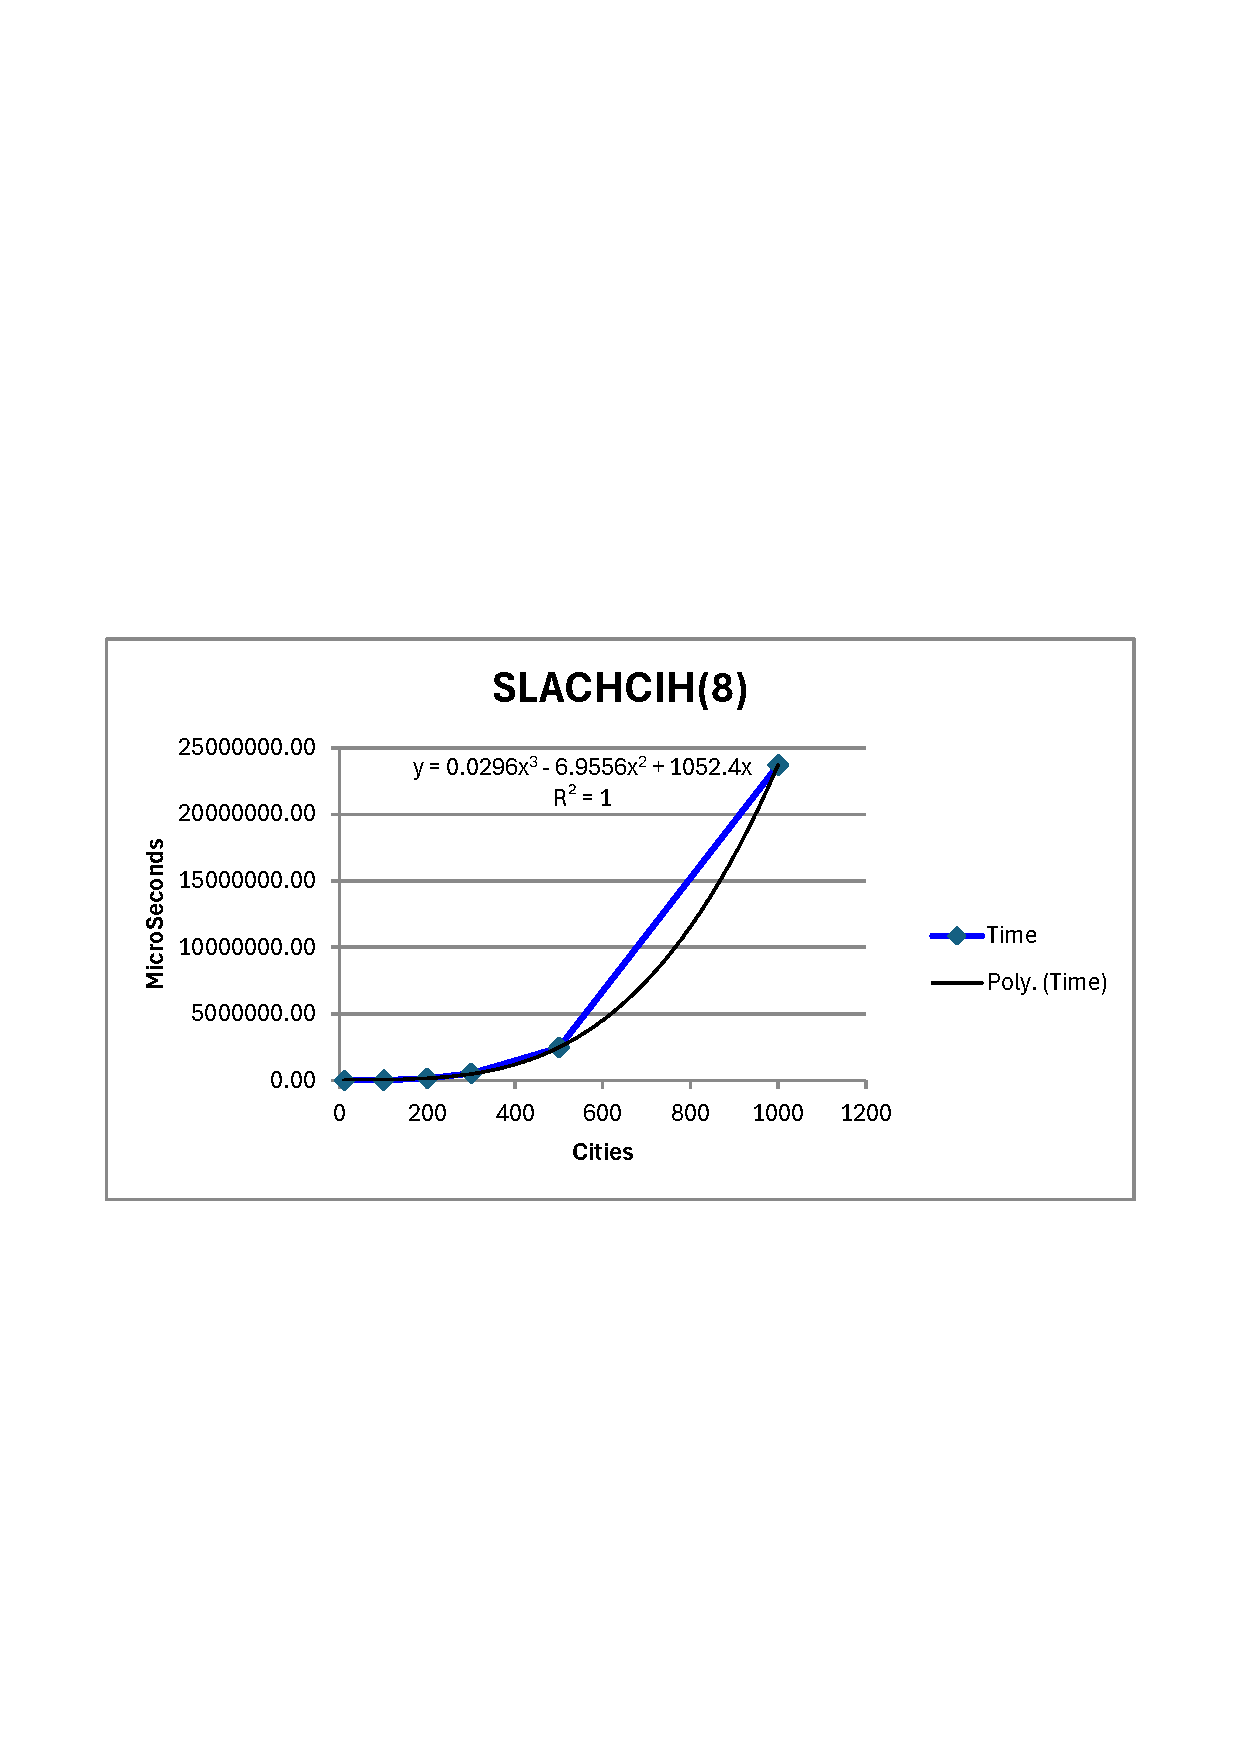
\includegraphics[width=0.8\textwidth]{sections/image/test_graph.pdf}
    \caption{SLACHCIH(8) Trend Line}
    \label{fig:timevssize}
\end{figure}

The value the look-ahead depth has is the difference between the algorithm time complexity being $O(n^3)$(when the depth is zero), and $O(n^5)$(when depth is $n$); this is the same as in Equation\ref{equ:statictime}. The CIH part of the algorithm is a constant $O(n^3)$ time complexity, while the look-ahead cost is based on the depth. This is observed in the data by changing the depths(Figure\ref{fig:timevsdepth}); the difference in time complexity is $O(n^2)$, which matches the cost of the look-ahead function.

The jump from depth zero to depth one is abrupt; this abnormally large increase is theorised as the cost of invoking the $ShortestRoute()$ function, which would only be fully invoked if depth is greater than 0. This is noticeable in Figure\ref{chart:depth} between the violet and indigo lines.
\begin{figure}[H]
    \centering
    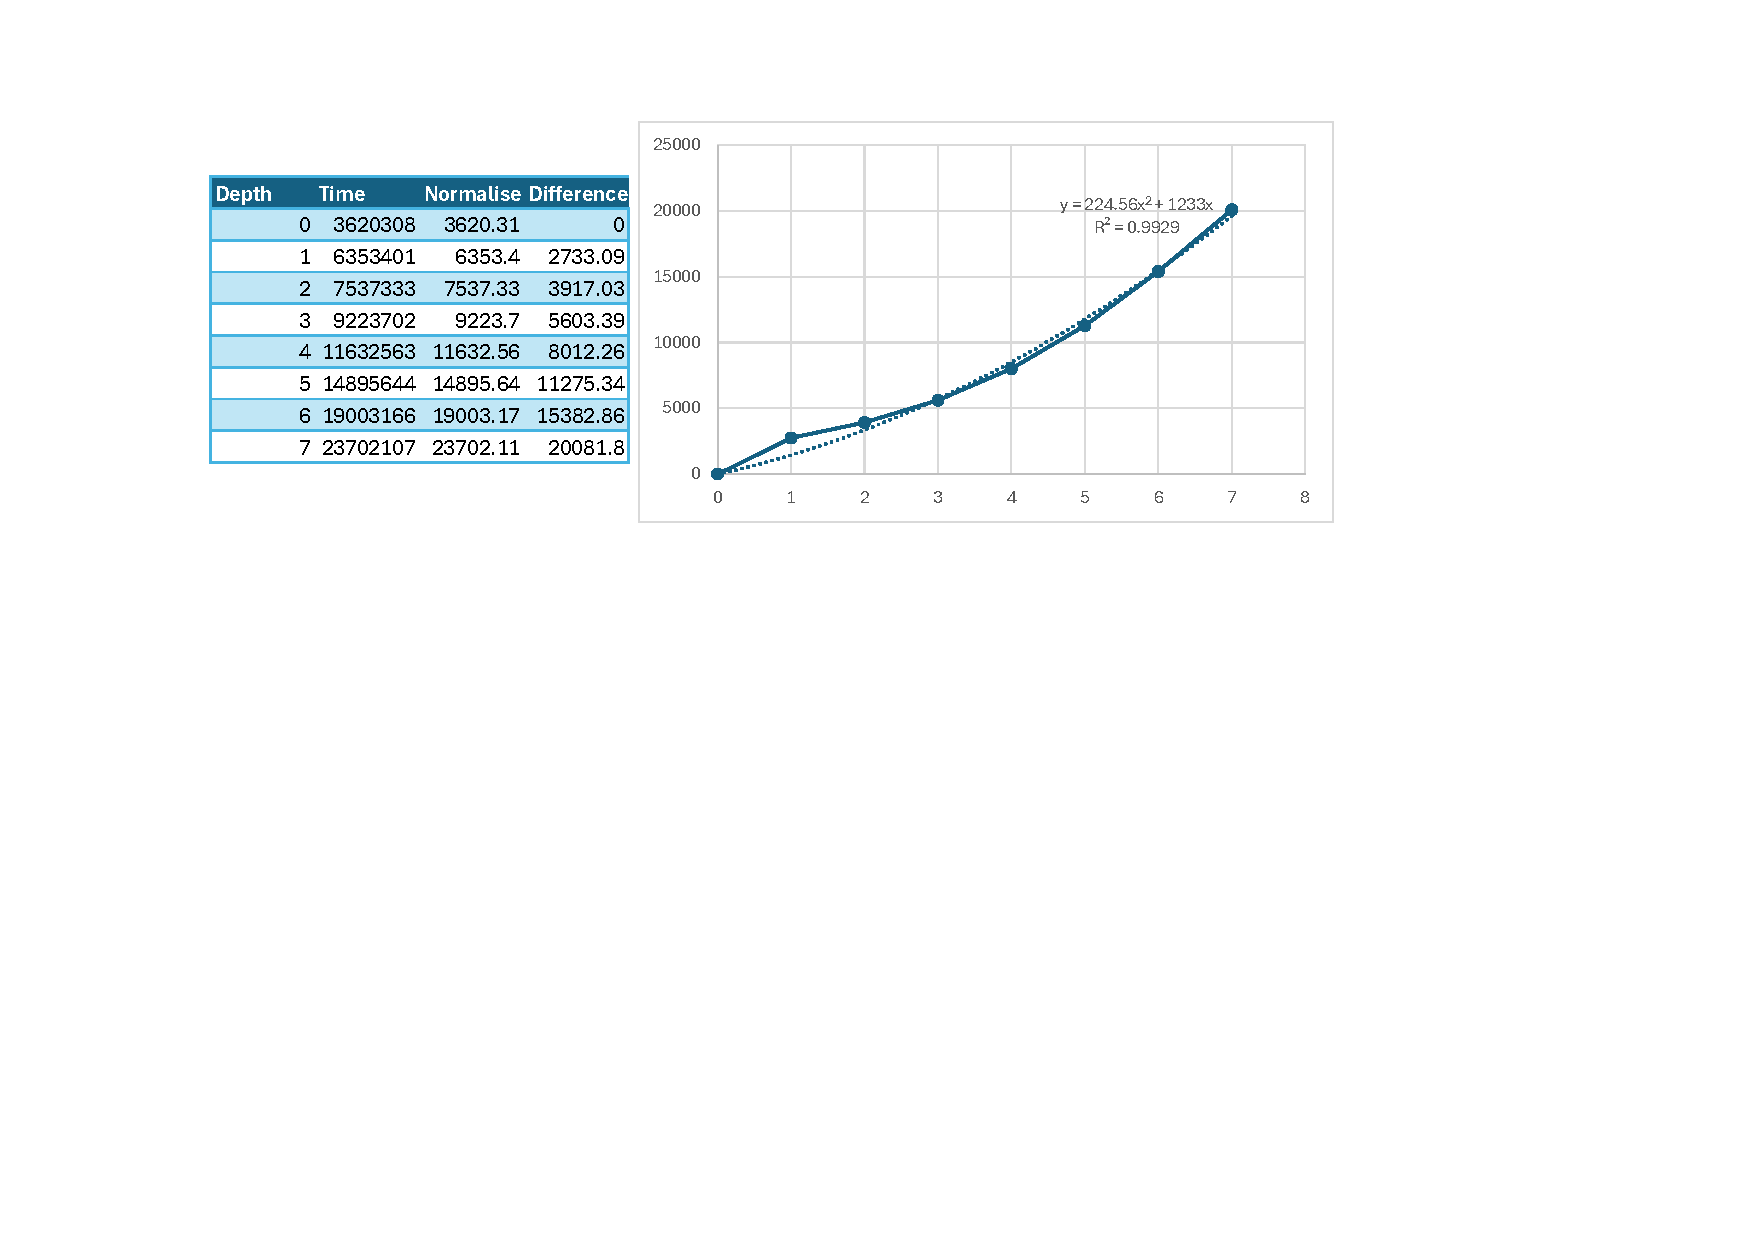
\includegraphics[width=\textwidth]{sections/image/test_graph2.pdf}
    \caption{Depth Trend Line}
    \label{fig:timevsdepth}
\end{figure}

\begin{figure}[H]
    \centering
    \resizebox{0.7\textwidth}{!}{%
    \begin{tikzpicture}
        \begin{axis}[
            xlabel={Problem Size}, 
            ylabel={MicroSeconds},
            title={Depth Vs Time},
            domain=1:1200, % Adjust range as needed
            samples=1000,
            grid=major,
            thick,
            legend style={at={(0.02,0.98)}, anchor=north west}, % Top-left corner
            legend entries={
                0 (Violet),
                1 (Indigo),
                2 (Blue),
                3 (Green),
                4 (Yellow),
                5 (Orange),
                6 (Red),
                7 (Black)
            }
        ]
    \addplot[violet] coordinates
      {(10,29) (100,5051) (200,36190) (300,111427) (500,488391)(1000,3620307)};

    \addplot[indigo] coordinates
      {(10,25.37) (100,7261.49) (200,48326.42) (300,155657.94) (500,689855.24)(1000,6353401.04)};

    \addplot[blue] coordinates
      {(10,24.09) (100,8234.30) (200,56582.62) (300,182868.75) (500,803808.43)(1000,7537333.35)};
      
      \addplot[green] coordinates
      {(10,24.06) (100,10040.87) (200,69633.18) (300,218068.36) (500,969888.68)(1000,9223702.34)};

      \addplot[yellow] coordinates
      {(10,24.41) (100,12184.33) (200,87280.23) (300,272952.20) (500,1220761.27)(1000,11632562.85)};
      
      \addplot[orange] coordinates
      {(10,24.44) (100,14956.88) (200,108331.81) (300,343997.62) (500,1542499.09)(1000,14895643.66)};

    \addplot[red] coordinates
      {(10,24.71) (100,17467.33) (200,134173.32) (300,432163.16) (500,1968387.66)(1000,19003165.87)};

      \addplot[black] coordinates
      {(10,24.18) (100,20843.73) (200,164704.99) (300,533267.40) (500,2469852.32)(1000,23702107.36)};


        \end{axis}
    \end{tikzpicture}
    }%
    \caption{Plot Of Depth Vs Time}
    \label{chart:depth}
\end{figure}